\chapter{The game as it plays: environment, cast, equipment and tactics}

Every photograph in this chapter was taken from the live place on 14 September
2026, by driving the Studio camera to the stated position and capturing the
viewport.\ Nothing is a mock-up or a render of a plan.\

\section{Photographic survey}

\begin{figure}[htbp]\centering
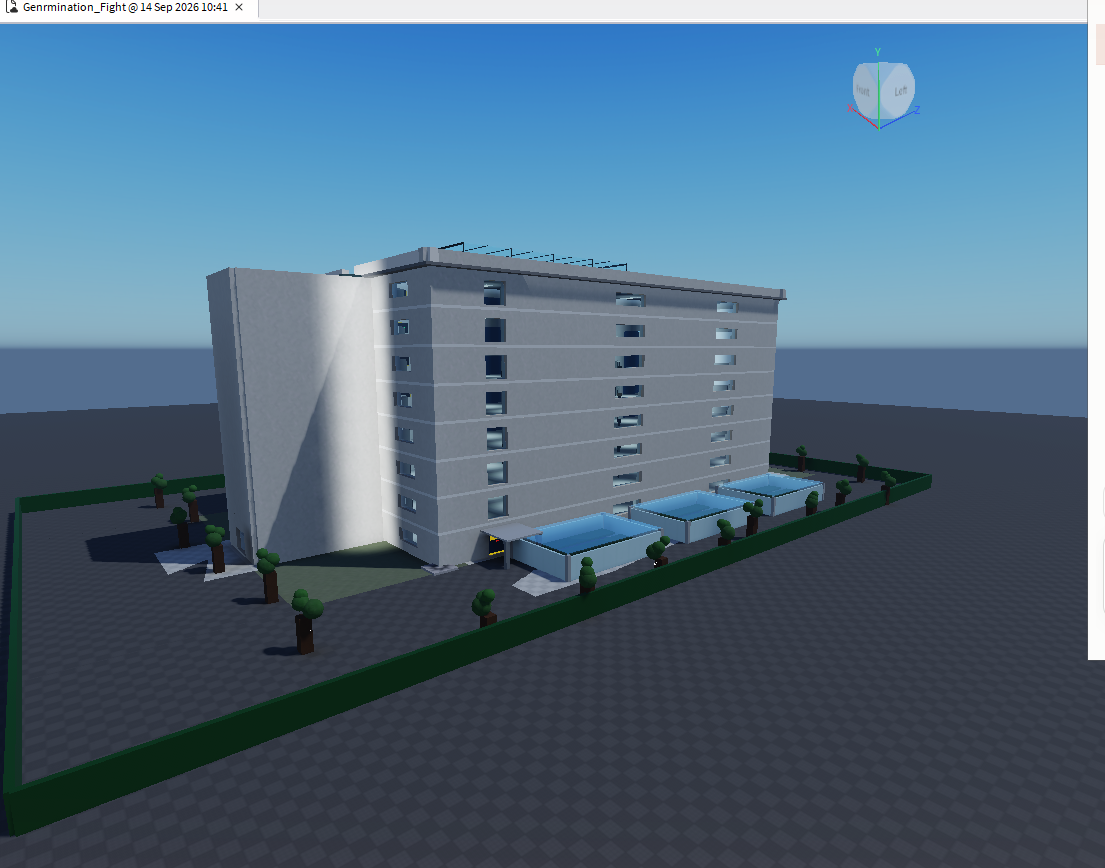
\includegraphics[width=0.92\textwidth]{figures/shots/fig01-exterior.png}
\caption{The laboratory from the south-west approach. Eight storeys above grade
over a basement, inside a fenced compound. The three blue-glazed structures on
the apron are the ground-level glasshouses; the darker strip at the near corner
is the entrance canopy.}
\end{figure}

\begin{figure}[htbp]\centering
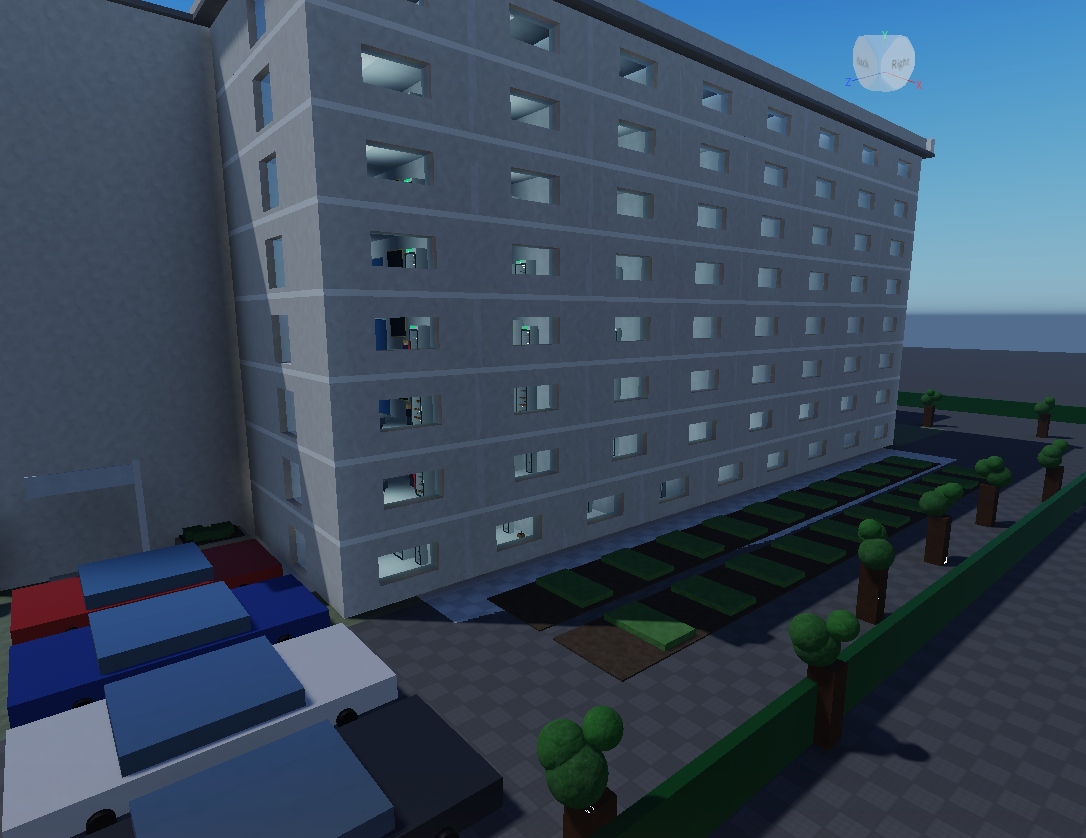
\includegraphics[width=0.92\textwidth]{figures/shots/fig02-siteworks.png}
\caption{Site works from the north-east: perimeter fence and gate, parking bays
with four vehicles, planters, flagpole, trial plots and twenty-eight trees
planted in bands that avoid the building footprint and the aprons.}
\end{figure}

\begin{figure}[htbp]\centering
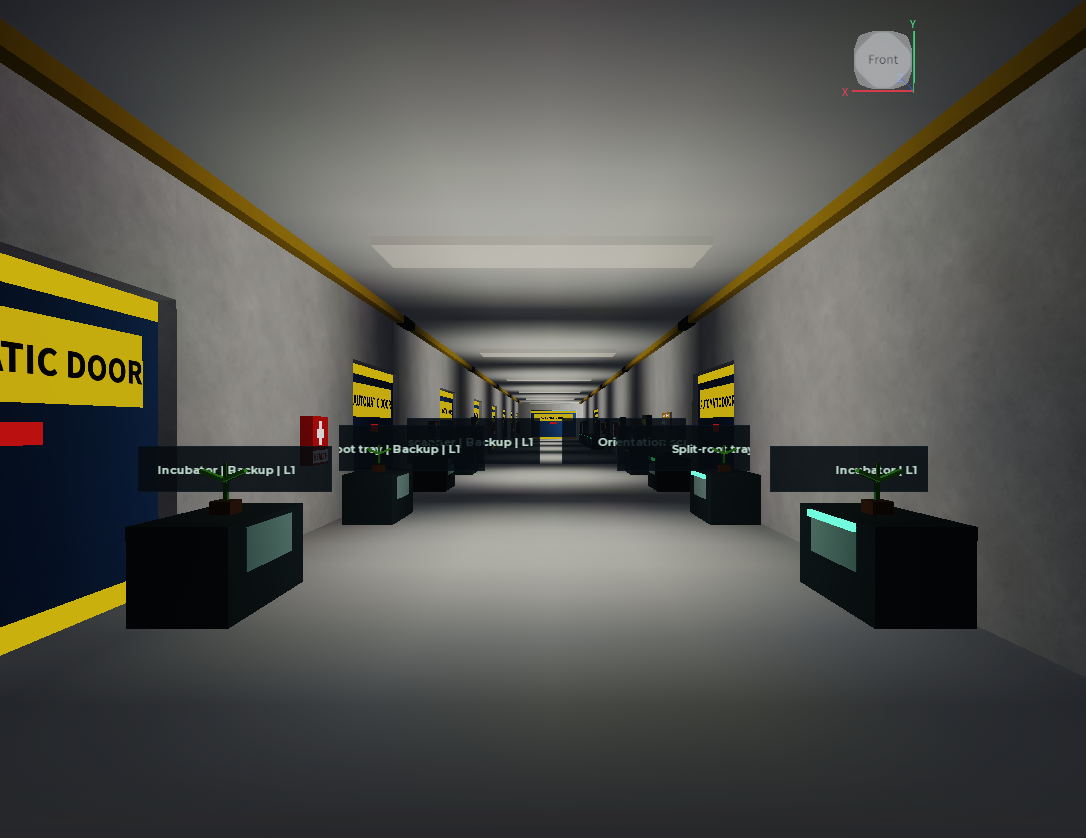
\includegraphics[width=0.92\textwidth]{figures/shots/fig03-corridor.png}
\caption{A typical floor corridor, looking north along Level 1. Research
stations stand against both walls with their own labels and status lights;
automatic doors are marked in yellow and blue; emergency kits are the red
cabinets. The corridor is the spine of every floor and the only continuous
route between the two stair towers.}
\end{figure}

\begin{figure}[htbp]\centering
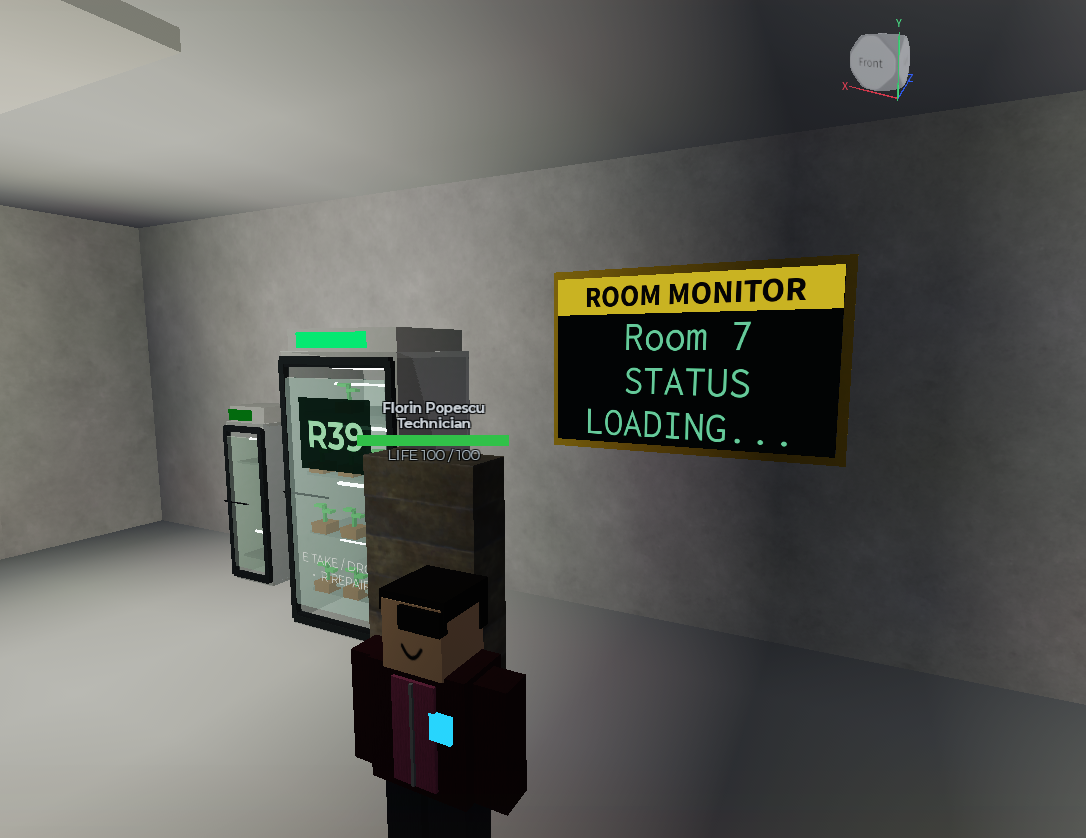
\includegraphics[width=0.92\textwidth]{figures/shots/fig04-growthchambers.png}
\caption{Inside a laboratory room. The germination chambers are the destructible
equipment: 450 of them across the building, each with its own growth code,
functional state and repair prompt.}
\end{figure}

\begin{figure}[htbp]\centering
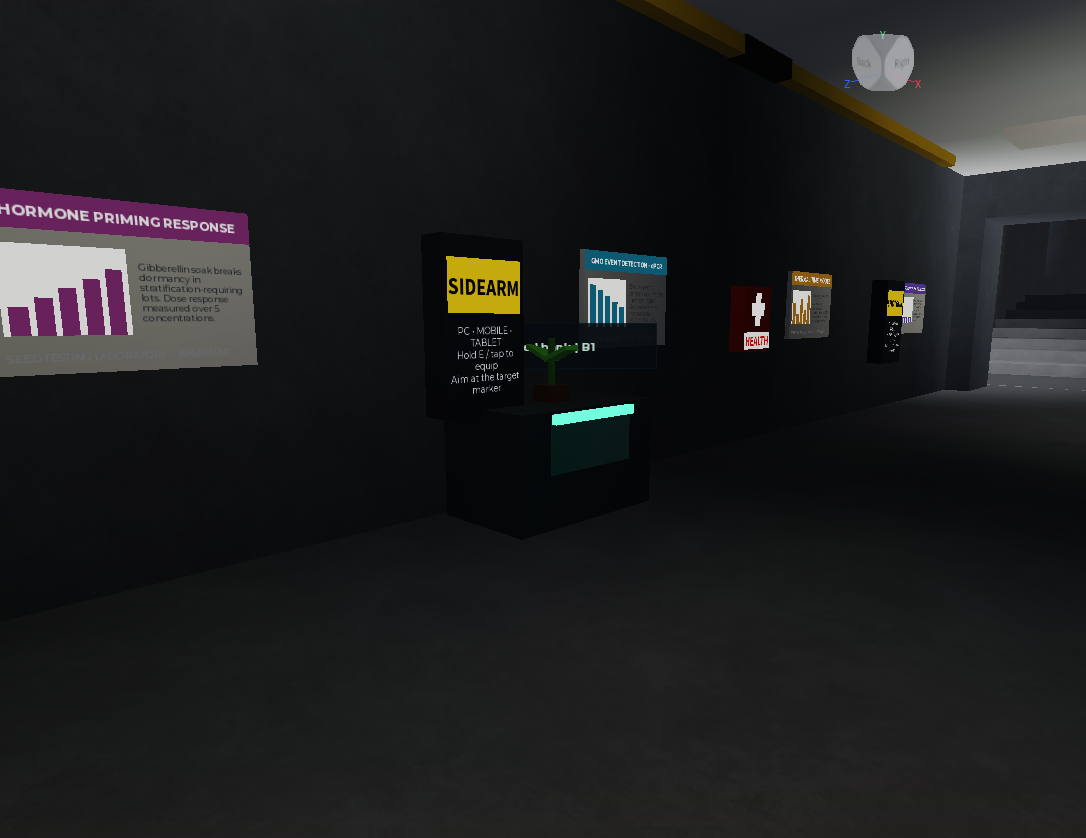
\includegraphics[width=0.92\textwidth]{figures/shots/fig05-seedbank.png}
\caption{The seed bank in the basement. This is the first stop of the
germination assignment and the origin of the mission seedling.}
\end{figure}

\begin{figure}[htbp]\centering
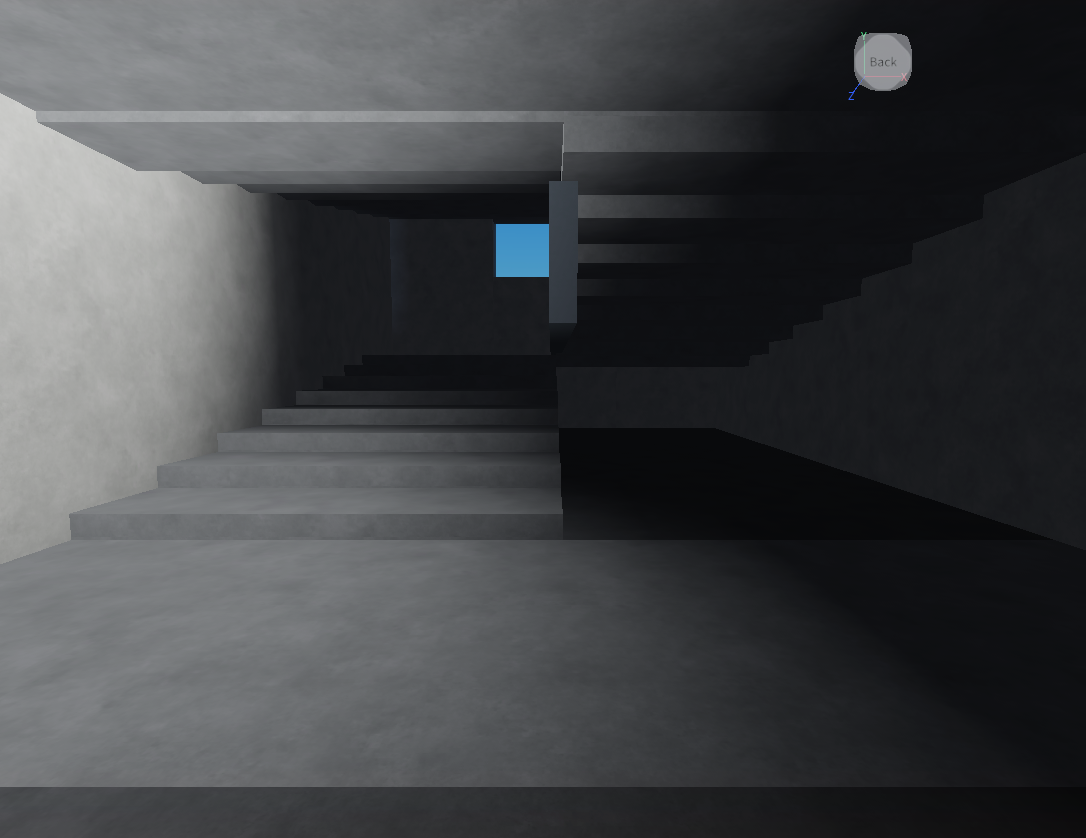
\includegraphics[width=0.92\textwidth]{figures/shots/fig06-basement-stairs.png}
\caption{The basement stair landing, after Revision 5 closed the void beneath
it. Before the repair this landing was a plate with nothing under it and a step
off the edge dropped the player out of the world.}
\end{figure}

\begin{figure}[htbp]\centering
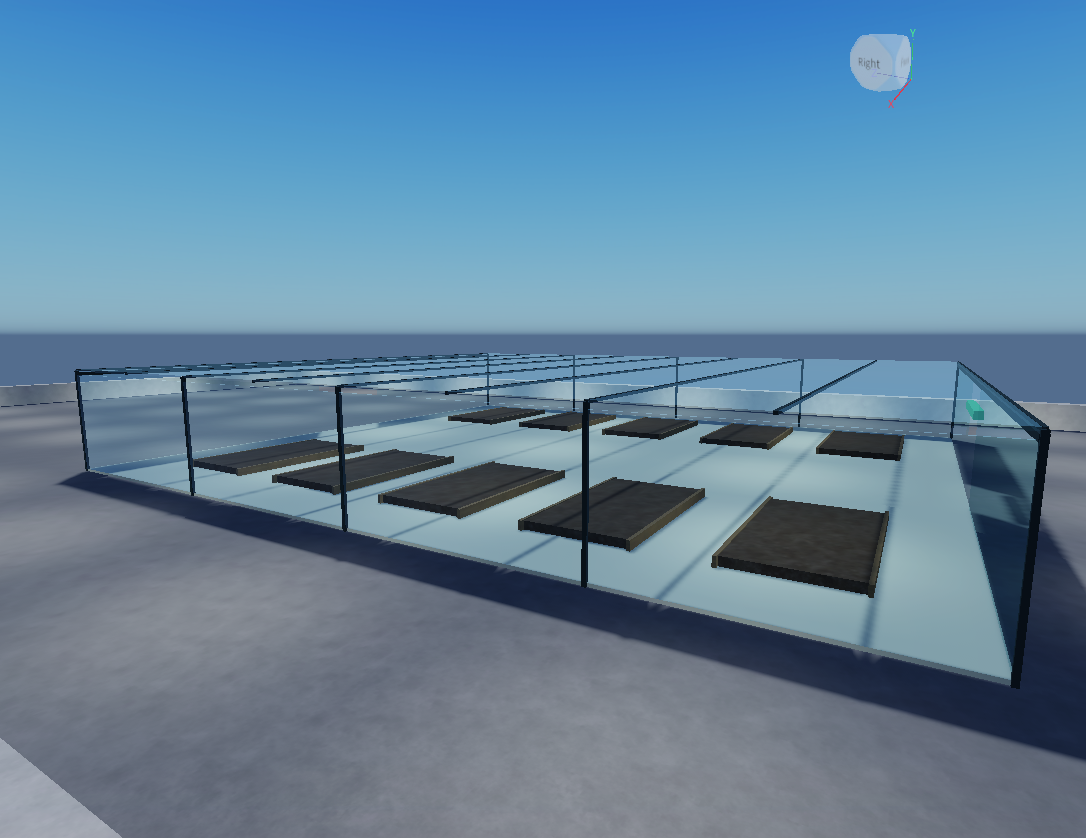
\includegraphics[width=0.92\textwidth]{figures/shots/fig07-greenhouse.png}
\caption{The rooftop greenhouse, the final stop of both assignments. Ten
planting plots sit under the glass; each accepts up to twelve seedlings.}
\end{figure}

\begin{figure}[htbp]\centering
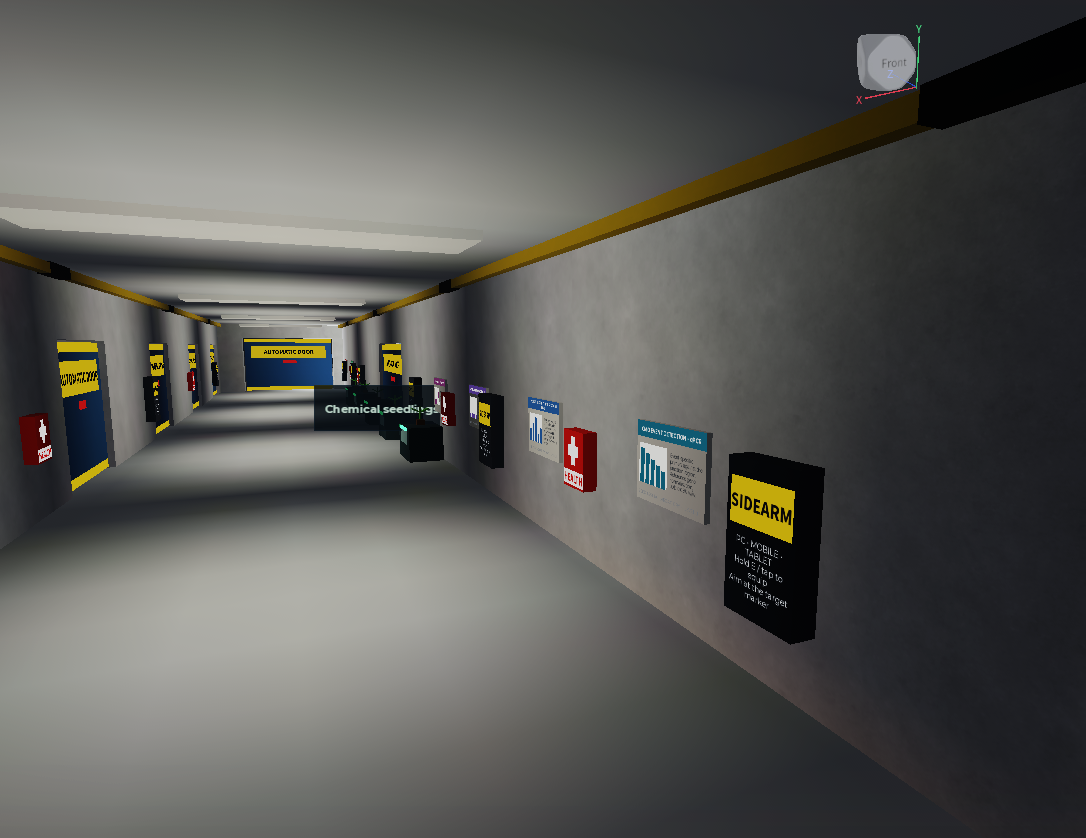
\includegraphics[width=0.92\textwidth]{figures/shots/fig08-fixtures.png}
\caption{Corridor fixtures: an emergency health kit, a weapon cabinet, a
scientific poster, and the yellow gas line running near the ceiling. The gas
line is live ordnance -- a shot into it detonates the section.}
\end{figure}

\begin{figure}[htbp]\centering
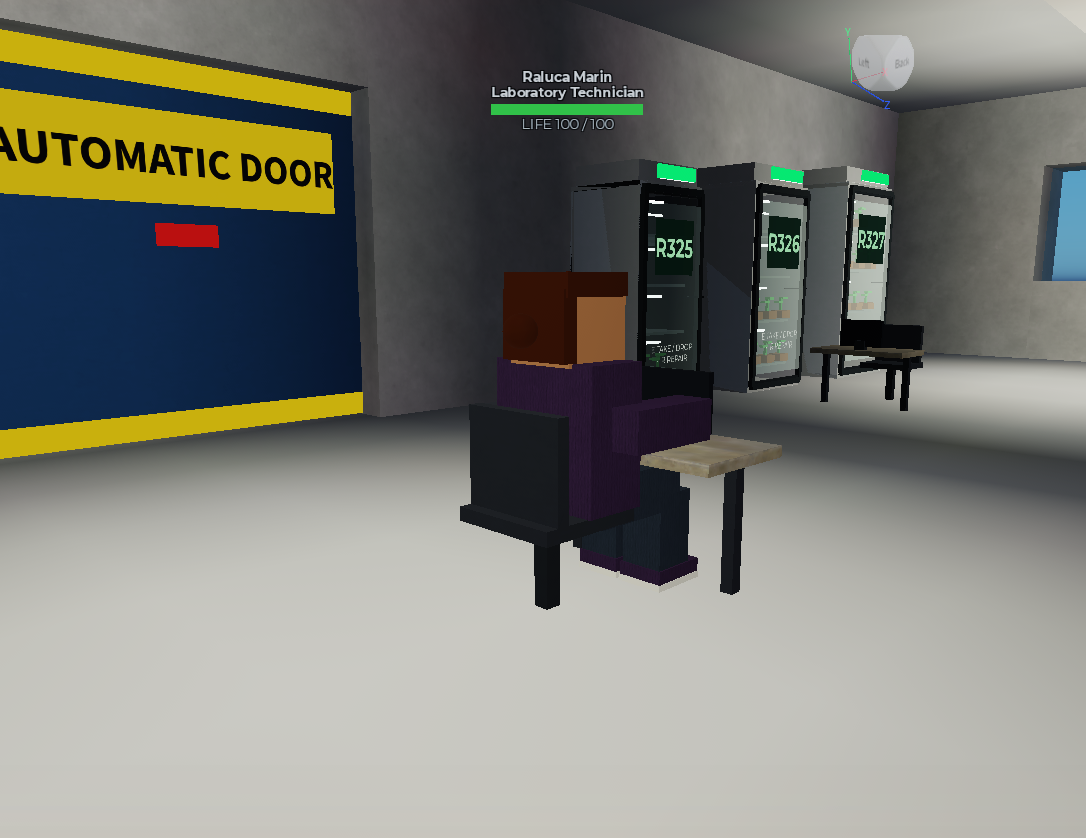
\includegraphics[width=0.92\textwidth]{figures/shots/fig09-seated-worker.png}
\caption{A seated worker at a workstation. Forty-five of the one hundred and
eighty workers are desk staff: they never patrol and never join an ambush, but
they are still targets.}
\end{figure}

\begin{figure}[htbp]\centering
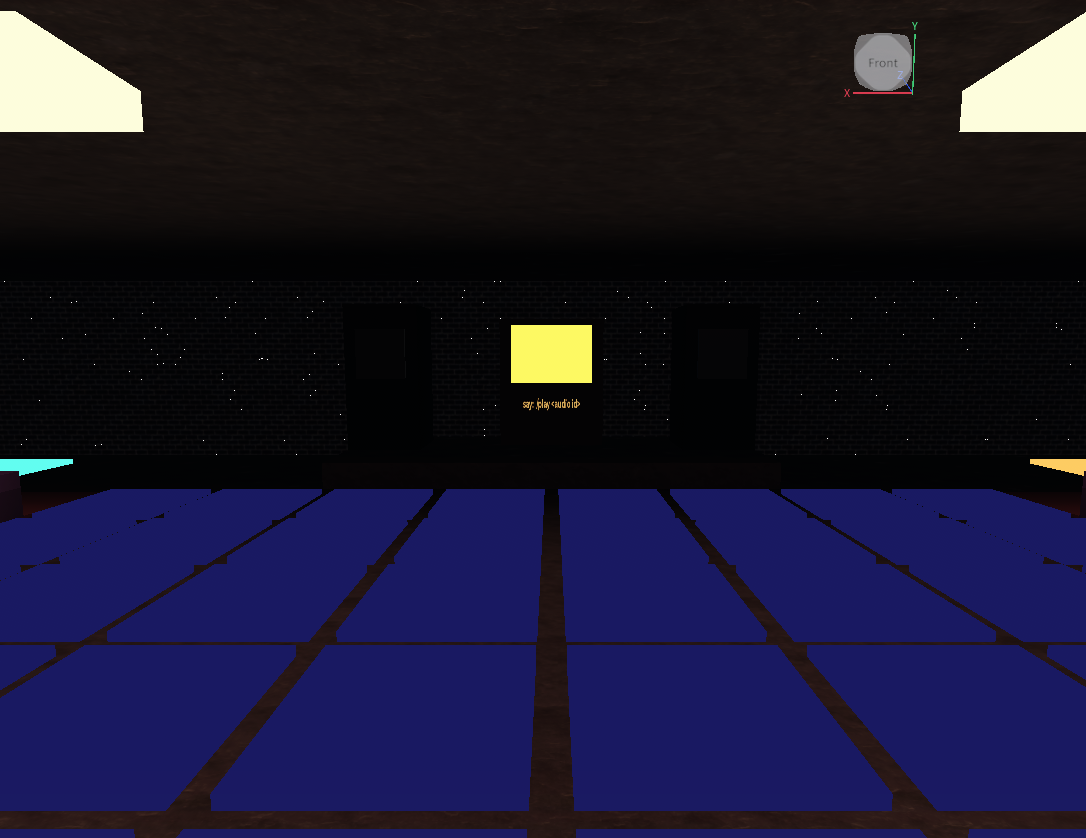
\includegraphics[width=0.92\textwidth]{figures/shots/fig11-lounge.png}
\caption{The hidden lounge, sealed beneath the basement and reached only through
the floor hatch. It has a bar, a stage, a jukebox and a message wall on which
players can post filtered notes.}
\end{figure}

\begin{figure}[htbp]\centering
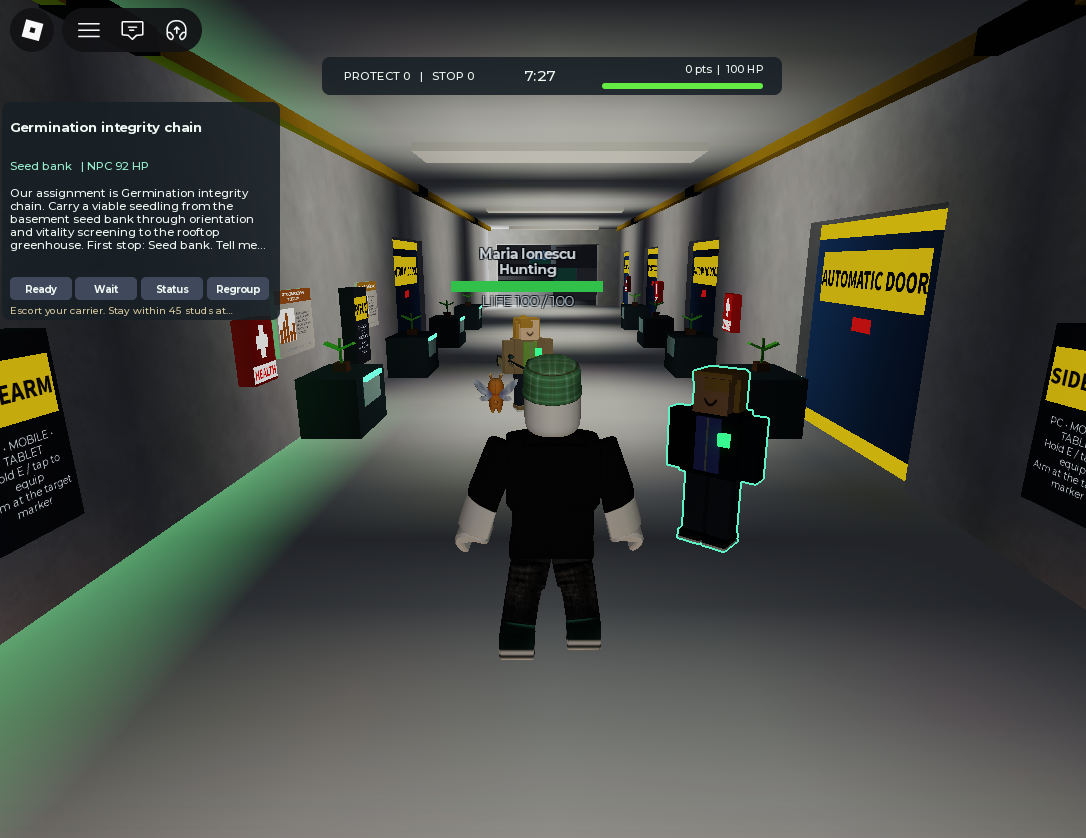
\includegraphics[width=0.92\textwidth]{figures/shots/fig12-hud-ingame.png}
\caption{Gameplay. The mission panel carries the assignment title, the current
stop, the carrier's health and the four carrier commands. The top strip shows
both role scores, the shift clock, points and player health. The green line on
the floor is the mission trail. The worker on the right is a live ambusher --
its billboard reads \emph{Hunting}, the state that tells the patrol system to
stand aside.}
\end{figure}

\begin{figure}[htbp]\centering
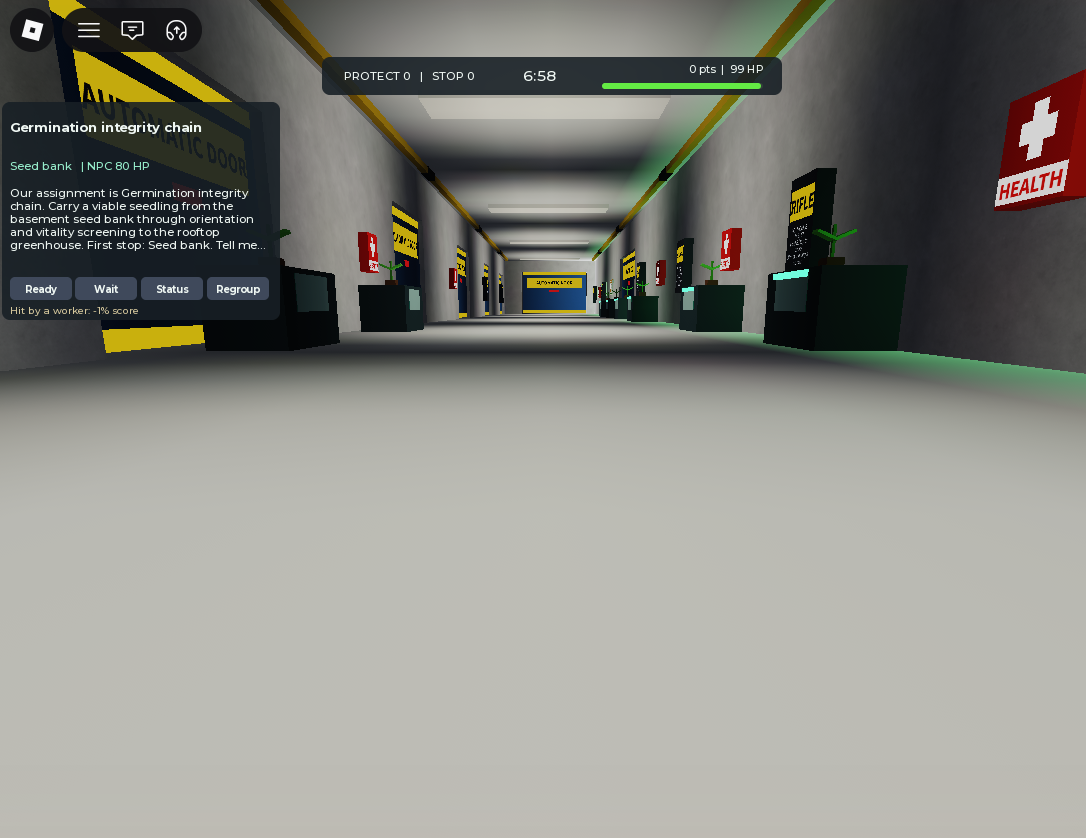
\includegraphics[width=0.92\textwidth,trim=0 430 0 0,clip]{figures/shots/fig13-ambush-standoff.png}
\caption{The same corridor during an ambush, from above and behind. Workers hold
a firing line rather than closing: none comes inside fifteen studs, which is
what makes them aimable.}
\end{figure}

\clearpage
\section{The environment}

\subsection{Scale}
The complex occupies roughly $326 \times 487$ studs in plan and stands 162 studs
from the basement floor to the roof parapet, an envelope of
$x\ -80\ldots246$, $y\ -17\ldots145$, $z\ -141\ldots346$.\ It is built from
61{,}694 parts.\ Nine occupied levels carry between 5{,}831 and 7{,}225 parts
each; the basement is the densest.\

\begin{center}
\begin{tabular}{@{}lr@{}}
\toprule
\textbf{Level} & \textbf{Parts} \\
\midrule
Basement & 7{,}225 \\
Level 1 & 5{,}831 \\
Level 2 & 6{,}140 \\
Level 3 & 5{,}987 \\
Level 4 & 6{,}122 \\
Level 5 & 6{,}005 \\
Level 6 & 6{,}133 \\
Level 7 & 6{,}020 \\
Level 8 & 6{,}123 \\
\bottomrule
\end{tabular}
\end{center}

\subsection{Floor layout}
Every floor is one central corridor with rooms either side.\ The corridor runs
north to south between the two stair towers; the room walls are pierced by
automatic doors that slide up into the header when anyone comes within eleven
studs and hold open for at least three seconds.\ There are 162 such doors.\
The corridor is where the fixtures live: emergency health kits, weapon
cabinets, posters, and the gas line near the ceiling.\

\subsection{Vertical circulation}
Two stair towers, north and south, project beyond the building footprint and
run the full height.\ Each level is served by a landing, a half-landing and two
flights of eight treads.\ There are no working elevators.\ The towers are the
only way between floors, which makes them the natural place to intercept a
carrier and the worst place to be caught by an ambush.\

\subsection{Ground level and the site}
Outside the building the compound holds a perimeter fence with a vehicle gate,
an entrance canopy on posts, parking bays with four cars, two planters, a
flagpole, three glasshouses on the western apron, two trial plots to the east,
and twenty-eight trees.\ The ground plane sits at $y=-8$, between the basement
floor at $-16.25$ and the first floor at $0$.\

\subsection{The rooftop greenhouse}
The roof carries a glazed greenhouse containing ten planting plots.\ Both
assignments end here.\ A plot accepts twelve seedlings before it is full.\ The
greenhouse glass is breakable, and hostile workers will deliberately shoot it
out to open a firing line.\

\subsection{The hidden lounge}
A sealed room sits below the basement, $y\ -49\ldots-30$, reached through a
hatch in the basement floor at $(110, -16, 130)$.\ It contains a bar with
stools, four sofa groups, a stage, a jukebox and a message wall.\ It is out of
play: no mission routes through it and no worker patrols there.\

\section{Characters}

\subsection{The two player roles}
Roles are chosen at one of two kiosks and cannot be changed mid-assignment.\

\begin{center}
\begin{tabular}{@{}p{0.22\textwidth}p{0.70\textwidth}@{}}
\toprule
\textbf{Role} & \textbf{Objective} \\
\midrule
Technician & Escort the research carrier to the rooftop greenhouse. Score for staying within 45 studs at each checkpoint, and for the final planting. Hitting your own carrier cancels your escort rewards. Only a Technician may repair destroyed equipment. \\
Laboratory Technician & Stop the carrier before it plants. Score for bringing it down. \\
\bottomrule
\end{tabular}
\end{center}

Selecting a role assigns one of the two missions immediately.\ There is no
mission menu.\

\subsection{Laboratory workers}
One hundred and eighty workers populate the building.\ They are differentiated
by appearance and name, and forty-five of them are seated desk staff who never
leave their workstation.\ The rest run a shift routine: they respond to
equipment alarms, walk between rooms, and idle when no player is in the room
with them -- an occupancy gate that keeps most of the roster asleep and is the
single largest reason the building runs at all.\

Workers become hostile only through the ambush system.\ At most five are armed
at any moment; when one is put down, a room further along the player's route
releases a replacement.\

\subsection{The research carrier}
The carrier is the mission.\ It is a worker rig that walks the assignment route
under navigation derived from the live map, carries the seedling between
stations, and speaks to its escort through the mission panel.\ It has 100 health
and no weapon.\ If it dies the round is decided in the Laboratory Technician's
favour and a fresh assignment is issued eight seconds later.\

\section{Equipment and fixtures}

\begin{center}
\begin{tabular}{@{}lrp{0.52\textwidth}@{}}
\toprule
\textbf{Fixture} & \textbf{Count} & \textbf{Behaviour} \\
\midrule
Germination chamber & 450 & Destructible. Explodes when shot, killing workers within 17 studs and hurting the player. A Technician restores it by holding R. \\
Research station & 67 & Twenty capabilities, each with an original and two backups, plus ten rooftop plots. Mission stops resolve to a capability, not a specific machine. \\
Automatic door & 162 & Slides open within 11 studs, holds 3 seconds, and can be forced open by an ambush. \\
Emergency health kit & 90 & Restores health, then recharges over 25 seconds. \\
Weapon cabinet & 90 & Dispenses one of the three player weapons. \\
Gas line & 18 & Two runs per floor near the ceiling. Detonates when shot, with a 26-stud blast. \\
Scientific poster & 72 & Takes permanent bullet holes. \\
Luminaire & 333 & Corridor and room lighting. \\
\bottomrule
\end{tabular}
\end{center}

\section{Weapons}
Three weapons are available to players.\ All three cost the shooter one percent
of their score per shot, and a head shot does double damage rather than an
instant kill.\ A worker has 100 health.\

\begin{center}
\begin{tabular}{@{}lrrrrr@{}}
\toprule
\textbf{Weapon} & \textbf{Damage} & \textbf{Pellets} & \textbf{Range} & \textbf{Cooldown} & \textbf{Shots to kill} \\
\midrule
Lab Sidearm & 34 & 1 & 240 & 0.32 s & 3 \\
Lab Shotgun & 12 & 6 & 110 & 0.85 s & 2 \\
Lab Rifle & 55 & 1 & 620 & 0.95 s & 2 \\
\bottomrule
\end{tabular}
\end{center}

The sidearm is the fastest cycling weapon and the only one that stays accurate
while moving.\ The shotgun's 72 damage assumes every pellet connects, which
holds only inside about twenty studs; beyond that it degrades quickly.\ The
rifle is the corridor and stairwell weapon: its 620-stud range covers the full
length of any floor.\

Hostile workers fire a single accurate ray with no spread, once every ten
seconds each, for half a health point per hit.\ Their danger is not the rifle
damage; it is what they do to the room around you.\

\section{Gameplay}

\subsection{The round}
A shift lasts 480 seconds -- eight minutes -- sized from the equipment count and
the mean distance between machines.\ When it ends, destroyed equipment is
repaired, planted seedlings are cleared, bodies are removed and the workers are
stood back up.\

\subsection{Scoring}
\begin{center}
\begin{tabular}{@{}lr@{}}
\toprule
\textbf{Event} & \textbf{Points} \\
\midrule
Protected a research checkpoint (Technician, within 45 studs) & +15 \\
Protected the rooftop planting (Technician) & +60 \\
Stopped the assigned carrier (Laboratory Technician) & +50 \\
Hit by a worker & $-1\%$ of current score \\
Firing any weapon & $-1\%$ of current score \\
\bottomrule
\end{tabular}
\end{center}

The one percent costs are proportional, so they bite hardest when you are
winning.\ A player sitting on a large score loses more per trigger pull than a
player starting out.\

\subsection{Scenario one: the escort, minute by minute}
\begin{center}
\begin{tabular}{@{}p{0.13\textwidth}p{0.79\textwidth}@{}}
\toprule
\textbf{Time} & \textbf{What happens} \\
\midrule
0:00 & Pick the Technician kiosk. The assignment is issued at once and a carrier walks to you. The mission panel names the first stop. \\
0:10 & Press \emph{Ready}. The carrier sets off for the basement seed bank and the green trail appears. \\
0:30 & First stair tower descent. This is the first ambush window: rooms you pass on the way to the stairs wake as you approach. \\
1:00 & Seed bank. The carrier processes for four seconds and takes the seedling. Stay within 45 studs to bank the checkpoint. \\
1:30--4:30 & Four more stops, spread across the basement, Levels 1 and 2. Expect at least one reroute: some stations have no walkable approach and the carrier will divert to a backup with the same capability. \\
5:00 & Long climb to the roof. The stair towers are where an opposing Laboratory Technician will wait, because the carrier cannot avoid them. \\
6:30 & Rooftop greenhouse. The carrier plants the seedling into a plot. Escort bonus awards if you are close. \\
7:00 & Assignment complete. A replacement is issued eight seconds later and the cycle restarts within the same shift. \\
8:00 & Shift ends. Equipment repairs, plots clear, workers stand back up. \\
\bottomrule
\end{tabular}
\end{center}

\subsection{Scenario two: the interception}
\begin{center}
\begin{tabular}{@{}p{0.13\textwidth}p{0.79\textwidth}@{}}
\toprule
\textbf{Time} & \textbf{What happens} \\
\midrule
0:00 & Pick the Laboratory Technician kiosk. You are assigned the cold-chain audit and a carrier of your own. \\
0:20 & Collect a rifle from a corridor cabinet. The rifle, not the shotgun: you will be shooting down corridors and stairwells. \\
1:00 & Locate the carrier. Its destination floor is on the mission panel, so you can move to the stairwell it must use rather than chase it. \\
2:00 & Take the stairwell. A carrier in a flight cannot leave it and cannot shoot back. \\
2:30 & Sustained fire brings it down in about 25 seconds unopposed; far less with the ambush helping, since half of every ambush targets the carrier. \\
3:00 & +50 points. A replacement carrier is issued, and you reposition for the next one. \\
\bottomrule
\end{tabular}
\end{center}

\section{Tactics worth knowing}
These are consequences of how the systems are built, verified by measurement.\
They are legitimate play, not defects, but they are not obvious.\

\begin{enumerate}
\item \textbf{Let the ambush kill the carrier for you.}\ Half of every ambush is
      assigned to the carrier when it wakes.\ As a Laboratory Technician you
      often do not need to fire at all -- shadow the carrier, stay out of the
      standoff line, and let the building do the work.\
\item \textbf{As a Technician, pull the ambush off the carrier.}\ Hostiles that
      are not carrier hunters switch to whoever is closest.\ Standing on the far
      side of the corridor from your carrier drags the other half of the roster
      onto you, which is survivable at half a point per hit.\
\item \textbf{Never fight next to a gas line.}\ Hostiles deliberately shoot
      pipes and machines near you.\ The blast radius is 26 studs for a pipe and
      17 for a machine, and both hurt you far more than a rifle round.\ Fight in
      the middle of the corridor, not against the wall where the fixtures are.\
\item \textbf{Weapon cost is proportional.}\ At 1\% of score per shot, a missed
      burst late in a round costs more than the same burst early.\ Once you are
      ahead, stop firing and escort.\
\item \textbf{Head shots are worth aiming for, but not decisive.}\ They double
      damage; they no longer kill outright.\ A rifle head shot still takes a
      worker down in one, a sidearm head shot does not.\
\item \textbf{Emergency kits recharge, so corridors are safe ground.}\ Ninety
      kits on a 25-second cycle means sustained hostile fire is survivable
      indefinitely if you keep moving between them.\
\item \textbf{Break the line of sight rather than the distance.}\ Hostiles hold
      at twenty studs and shoot accurately, but they will not close.\ Stepping
      into a room and letting the door shut ends the engagement outright.\
\item \textbf{Repair is a scoring move for Technicians.}\ Destroyed equipment
      removes a station from the mission pool and can force a reroute.\ Repairing
      it near a carrier's next stop shortens the route.\
\item \textbf{Stairwells favour the interceptor.}\ A carrier on a flight follows
      the treads and cannot deviate, which makes its position predictable for
      several seconds.\
\item \textbf{The rooftop is the last chance, not the best one.}\ Hostiles will
      shoot out the greenhouse glass to reach you, so cover there is temporary.\
\end{enumerate}
